\documentclass[10pt,ignorenonframetext,]{beamer}
\setbeamertemplate{caption}[numbered]
\setbeamertemplate{caption label separator}{: }
\setbeamercolor{caption name}{fg=normal text.fg}
\beamertemplatenavigationsymbolsempty
\usepackage{lmodern}
\usepackage{amssymb,amsmath}
\usepackage{ifxetex,ifluatex}
\usepackage{fixltx2e} % provides \textsubscript
\ifnum 0\ifxetex 1\fi\ifluatex 1\fi=0 % if pdftex
  \usepackage[T1]{fontenc}
  \usepackage[utf8]{inputenc}
\else % if luatex or xelatex
  \ifxetex
    \usepackage{mathspec}
  \else
    \usepackage{fontspec}
  \fi
  \defaultfontfeatures{Ligatures=TeX,Scale=MatchLowercase}
\fi
\usetheme[]{Singapore}
\usefonttheme{serif}
% use upquote if available, for straight quotes in verbatim environments
\IfFileExists{upquote.sty}{\usepackage{upquote}}{}
% use microtype if available
\IfFileExists{microtype.sty}{%
\usepackage{microtype}
\UseMicrotypeSet[protrusion]{basicmath} % disable protrusion for tt fonts
}{}
\newif\ifbibliography
\hypersetup{
            pdftitle={Module 9: Support Vector Machines},
            pdfauthor={Stefanie Muff, Department of Mathematical Sciences, NTNU},
            colorlinks=true,
            linkcolor=Maroon,
            citecolor=Blue,
            urlcolor=blue,
            breaklinks=true}
\urlstyle{same}  % don't use monospace font for urls
\usepackage{color}
\usepackage{fancyvrb}
\newcommand{\VerbBar}{|}
\newcommand{\VERB}{\Verb[commandchars=\\\{\}]}
\DefineVerbatimEnvironment{Highlighting}{Verbatim}{commandchars=\\\{\}}
% Add ',fontsize=\small' for more characters per line
\usepackage{framed}
\definecolor{shadecolor}{RGB}{248,248,248}
\newenvironment{Shaded}{\begin{snugshade}}{\end{snugshade}}
\newcommand{\KeywordTok}[1]{\textcolor[rgb]{0.13,0.29,0.53}{\textbf{#1}}}
\newcommand{\DataTypeTok}[1]{\textcolor[rgb]{0.13,0.29,0.53}{#1}}
\newcommand{\DecValTok}[1]{\textcolor[rgb]{0.00,0.00,0.81}{#1}}
\newcommand{\BaseNTok}[1]{\textcolor[rgb]{0.00,0.00,0.81}{#1}}
\newcommand{\FloatTok}[1]{\textcolor[rgb]{0.00,0.00,0.81}{#1}}
\newcommand{\ConstantTok}[1]{\textcolor[rgb]{0.00,0.00,0.00}{#1}}
\newcommand{\CharTok}[1]{\textcolor[rgb]{0.31,0.60,0.02}{#1}}
\newcommand{\SpecialCharTok}[1]{\textcolor[rgb]{0.00,0.00,0.00}{#1}}
\newcommand{\StringTok}[1]{\textcolor[rgb]{0.31,0.60,0.02}{#1}}
\newcommand{\VerbatimStringTok}[1]{\textcolor[rgb]{0.31,0.60,0.02}{#1}}
\newcommand{\SpecialStringTok}[1]{\textcolor[rgb]{0.31,0.60,0.02}{#1}}
\newcommand{\ImportTok}[1]{#1}
\newcommand{\CommentTok}[1]{\textcolor[rgb]{0.56,0.35,0.01}{\textit{#1}}}
\newcommand{\DocumentationTok}[1]{\textcolor[rgb]{0.56,0.35,0.01}{\textbf{\textit{#1}}}}
\newcommand{\AnnotationTok}[1]{\textcolor[rgb]{0.56,0.35,0.01}{\textbf{\textit{#1}}}}
\newcommand{\CommentVarTok}[1]{\textcolor[rgb]{0.56,0.35,0.01}{\textbf{\textit{#1}}}}
\newcommand{\OtherTok}[1]{\textcolor[rgb]{0.56,0.35,0.01}{#1}}
\newcommand{\FunctionTok}[1]{\textcolor[rgb]{0.00,0.00,0.00}{#1}}
\newcommand{\VariableTok}[1]{\textcolor[rgb]{0.00,0.00,0.00}{#1}}
\newcommand{\ControlFlowTok}[1]{\textcolor[rgb]{0.13,0.29,0.53}{\textbf{#1}}}
\newcommand{\OperatorTok}[1]{\textcolor[rgb]{0.81,0.36,0.00}{\textbf{#1}}}
\newcommand{\BuiltInTok}[1]{#1}
\newcommand{\ExtensionTok}[1]{#1}
\newcommand{\PreprocessorTok}[1]{\textcolor[rgb]{0.56,0.35,0.01}{\textit{#1}}}
\newcommand{\AttributeTok}[1]{\textcolor[rgb]{0.77,0.63,0.00}{#1}}
\newcommand{\RegionMarkerTok}[1]{#1}
\newcommand{\InformationTok}[1]{\textcolor[rgb]{0.56,0.35,0.01}{\textbf{\textit{#1}}}}
\newcommand{\WarningTok}[1]{\textcolor[rgb]{0.56,0.35,0.01}{\textbf{\textit{#1}}}}
\newcommand{\AlertTok}[1]{\textcolor[rgb]{0.94,0.16,0.16}{#1}}
\newcommand{\ErrorTok}[1]{\textcolor[rgb]{0.64,0.00,0.00}{\textbf{#1}}}
\newcommand{\NormalTok}[1]{#1}
\usepackage{graphicx,grffile}
\makeatletter
\def\maxwidth{\ifdim\Gin@nat@width>\linewidth\linewidth\else\Gin@nat@width\fi}
\def\maxheight{\ifdim\Gin@nat@height>\textheight0.8\textheight\else\Gin@nat@height\fi}
\makeatother
% Scale images if necessary, so that they will not overflow the page
% margins by default, and it is still possible to overwrite the defaults
% using explicit options in \includegraphics[width, height, ...]{}
\setkeys{Gin}{width=\maxwidth,height=\maxheight,keepaspectratio}

% Prevent slide breaks in the middle of a paragraph:
\widowpenalties 1 10000
\raggedbottom

\AtBeginPart{
  \let\insertpartnumber\relax
  \let\partname\relax
  \frame{\partpage}
}
\AtBeginSection{
  \ifbibliography
  \else
    \let\insertsectionnumber\relax
    \let\sectionname\relax
    \frame{\sectionpage}
  \fi
}
\AtBeginSubsection{
  \let\insertsubsectionnumber\relax
  \let\subsectionname\relax
  \frame{\subsectionpage}
}

\setlength{\parindent}{0pt}
\setlength{\parskip}{6pt plus 2pt minus 1pt}
\setlength{\emergencystretch}{3em}  % prevent overfull lines
\providecommand{\tightlist}{%
  \setlength{\itemsep}{0pt}\setlength{\parskip}{0pt}}
\setcounter{secnumdepth}{0}
\usepackage{multirow}

\title{Module 9: Support Vector Machines}
\subtitle{TMA4268 Statistical Learning V2020}
\author{Stefanie Muff, Department of Mathematical Sciences, NTNU}
\date{March xx, 2020}

\begin{document}
\frame{\titlepage}

\begin{frame}{Introduction}

This field dates back to the 1990s in computer science, and in this
presentation we put emphasis on the underlying motivation and
connections to linear algebra, optimization theory and statistics.

We will only cover classification, and in particular two-class problems.

\begin{block}{Learning material for this module}

\begin{itemize}
\tightlist
\item
  James et al (2013): An Introduction to Statistical Learning. Chapter
  9.\\
\item
  \href{https://www.math.ntnu.no/emner/TMA4268/2019v/notes/M9notes.pdf}{Classnotes
  11.03.2019} (Todo: Replace this by saying there will be classnotes
  e.g.~on the board)
\end{itemize}

\vspace{2mm} \small
Some of the figures in this presentation are taken from (or are inspired
by) James et al. (2013) with permission from the authors: G. James, D.
Witten, T. Hastie and R. Tibshirani.

\end{block}

\end{frame}

\begin{frame}

\begin{block}{Topics}

\begin{itemize}
\tightlist
\item
  Motivation
\item
  Maximal margin classifier
\item
  Support vector classifier
\item
  Support vector machines
\item
  Extensions
\item
  Comparisons
\item
  Summing up
\end{itemize}

\end{block}

\end{frame}

\begin{frame}

\begin{block}{Motivating example}

\begin{itemize}
\item
  Suppose that you are interested in the distribution of two tree types:
  redwood and pines.
\item
  You have three different study areas in which these trees grow.
\item
  Your study areas with the tree positions in three forests is
  visualized in the figures below. Orange: redwood tree; green: pine
  tree.
\end{itemize}

\begin{center}\includegraphics[width=0.8\linewidth]{9SVM_files/figure-beamer/trees-1} \end{center}

\vspace{-4mm}

\begin{itemize}
\tightlist
\item
  You want to build one continuous fence to separate the two tree types
  in each of the three study areas. \textbf{Where should you build the
  fence?}
\end{itemize}

\end{block}

\end{frame}

\begin{frame}

Three cases: \vspace{2mm}

\begin{itemize}
\item
  Forest 1 seems easy: The orange and green points are clearly separated
  and the fence can be built anywhere inside the band that separates
  them. However, we can draw infinitely many straight lines that all
  separate the two tree types, and we should take into account that the
  trees reproduce and that we want future pines and future redwoods to
  grow up on the correct side of the fence.
\item
  Forest 2 is a bit more complicated: A linear fence still seems like a
  good idea, but in this case the two tree types cannot be perfectly
  separated. You have to allow some of the trees to be on the wrong side
  of the fence.
\item
  Forest 3 is the most complex: It is not possible to separate the two
  tree types by a straight line without getting a large number of
  misclassifications. Here, a circular fence around the pine trees seems
  like a reasonable choice.
\end{itemize}

\end{frame}

\begin{frame}

Forest 1 illustrates the problem of finding an \textbf{optimal
separating hyperplane} for a dataset.

Topic: \textbf{Maximal Margin hyperplanes}

\begin{center}\includegraphics[width=0.5\linewidth]{9SVM_files/figure-beamer/forest1-1} \end{center}

\end{frame}

\begin{frame}

You are also going to learn how you can find an optimal separating
hyperplane when your data cannot be perfectly separated by a straight
line, as in Forest 2.

Topic: \textbf{Support Vector Classifier} or \textbf{Soft Margin
Classifier}

\begin{center}\includegraphics[width=0.5\linewidth]{9SVM_files/figure-beamer/forest2-1} \end{center}

\end{frame}

\begin{frame}

The Support vector classifier can be generalised to an approach that
produces non-linear decision boundaries. This is useful when the data is
distributed as illustrated in Forest 3.

Topic: \textbf{Support Vector Machines} (SVMs)

\begin{center}\includegraphics[width=0.5\linewidth]{9SVM_files/figure-beamer/forest3-1} \end{center}

\end{frame}

\begin{frame}

Why are we interested in an optimal hyperplane or a separating curve?

\(\rightarrow\) We want to use it for classification.

\begin{itemize}
\item
  In our example: Is it likely that a random seed found at location
  \((0.8,0.4)\) becomes a redwood or a pine tree given the observed
  data?
\item
  Classification of a new observation based on which side of the
  decision boundary it falls into.
\end{itemize}

\vspace{2mm}

\textbf{Note}: In this module we look at \textbf{binary classification},
but extensions to more than two classes are briefly mentioned.

\end{frame}

\begin{frame}

\begin{itemize}
\item
  We will use the three forests example throughout this module.
\item
  The two covaraites (\(x_1\), \(x_2\)) are the coordinates of the
  trees.
\item
  The response is either \(pine\) (\(y=1\)) or \(redwood\) (\(y=-1\)).
\item
  \textbf{Goal}: to make a classifier for random seeds that we find on
  the ground for each of the three forests. The locations of the seeds
  are shown in the figure below (black circles).
\end{itemize}

\end{frame}

\begin{frame}

\begin{itemize}
\item
  The point patterns of the known locations can be thought of as the
  training set.
\item
  The point pattern generated by the black circles can be thought of as
  the test set.
\end{itemize}

\begin{center}\includegraphics[width=0.9\linewidth]{9SVM_files/figure-beamer/trees2-1} \end{center}

\end{frame}

\begin{frame}{Maximal Margin Classifier}

\begin{block}{Hyperplane}

\vspace{2mm}

A \textbf{hyperplane} in p-dimensions is defined as

\[\beta_0+\beta_1 X_1 + \beta_2 X_2 +...+\beta_p X_p=\beta_0+{\boldsymbol x}^T {\boldsymbol \beta}=0.\]
and is a \(p-1\) dimensional subspace of \(\mathbb{R}^p\). \vspace{3mm}

\textbf{Recap}:

\begin{itemize}
\item
  If a point \({\boldsymbol x}=(x_1,x_2,...,x_p)^T\) satisfies the above
  equation, it lies on the hyperplane.
\item
  If \(\beta_0=0\) the hyperplane goes through the origin.
\item
  The vector \({\boldsymbol \beta}=(\beta_1, \ldots, \beta_p)\) (not
  including \(\beta_0\)) is called the normal vector and points in the
  direction orthogonal to the hyperplane.
\end{itemize}

\end{block}

\end{frame}

\begin{frame}

If a point \({\boldsymbol x}\) satisfies

\begin{itemize}
\item
  \(\beta_0+ {\boldsymbol \beta}^\top {\boldsymbol x}>0\) it lies on one
  side of the hyperplane
\item
  \(\beta_0+{\boldsymbol \beta}^\top {\boldsymbol x}<0\) it lies on the
  opposite side of the hyperplane.
\item
  \(\beta_0+{\boldsymbol \beta}^\top {\boldsymbol x}=0\) it lies on the
  hyperplane (by definition!).
\end{itemize}

\vspace{2mm}

\begin{itemize}
\item
  The signed distance of any point \(\boldsymbol x\) to the hyperplane
  is given by
  \[\frac{1}{||{\boldsymbol\beta}||} (\beta_0 + {\boldsymbol \beta}^\top {\boldsymbol x} )\ ,\]
  where \(||{\boldsymbol\beta}||^2 = \sum_{j=1}^p \beta_j^2=1\) is the
  (squared) length of \(\boldsymbol \beta\) (Euclidian norm).
\item
  See board for a graphical description (todo).
\end{itemize}

\end{frame}

\begin{frame}

\begin{block}{Assumptions}

\vspace{2mm}

\begin{itemize}
\item
  Assume that we have \(n\) training observations with \(p\) predictors
  \[{\boldsymbol x}_1=\left(
  \begin{array}{c}
    x_{11} \\
    \vdots \\
    x_{1p}
    \end{array}
    \right), \ldots, {\boldsymbol x}_n=\left(
  \begin{array}{c}
    x_{n1} \\
    \vdots \\
    x_{np}
    \end{array}
    \right)\]
\item
  The responses \(\boldsymbol{y}\) fall into two classes
  \(y_1,...,y_n \in \{-1,1\}\).
\item
  It is possible to separate the training observations perfectly
  according to their class.
\end{itemize}

\end{block}

\end{frame}

\begin{frame}

\begin{block}{Possible hyperplanes (Forest 1)}

\vspace{2mm} Which is ``best''?

\begin{center}\includegraphics[width=0.6\linewidth]{9SVM_files/figure-beamer/forest1.1-1} \end{center}

\end{block}

\end{frame}

\begin{frame}

\begin{block}{Classification with a simple hyperplane}

\vspace{2mm}

The three lines displayed in the figure are three possible separating
hyperplanes for this dataset which contains two predictors \(x_1\) and
\(x_2\) (\(p=2\)). The hyperplanes have the property that

\[\beta_0+\beta_1 x_{i1} + \beta_2 x_{i2}+...+\beta_p x_{ip}=\beta_0+{\boldsymbol x}_i^T {\boldsymbol \beta}>0\]

if \(y_i=1\) (green points) and

\[\beta_0+\beta_1 x_{i1} + \beta_2 x_{i2}+...+\beta_p x_{ip}=\beta_0+{\boldsymbol x}_i^T {\boldsymbol \beta}<0\]

if \(y_i=-1\) (orange points).

\end{block}

\end{frame}

\begin{frame}

This means that for all observations (all are correctly classified)

\[y_i (\beta_0+{\boldsymbol x}_i^T {\boldsymbol \beta})>0 \ .\]

\vspace{2mm} The hyperplane thus leads to a
\emph{\textcolor{red}{natural classifier}}, depending on the side of the
hyperplane where the new observation lies.

The class \(y^*\) of a new observation \(x^*=(x_1^*,...,x_n^*)\) is
assigned depending on the value
\(f(x^*)=\beta_0+\beta_1 x_1^* + \beta_2 x_{2}^*+...+\beta_p x_{p}^*\)

\begin{center}
\colorbox{lightgray}{\begin{minipage}{8cm}
{\bf Hyperplane classifier:}

$$y^* = \left\{ \begin{array}{ll}
1 \ , & \text{if } f(x^*) >0 \ ,\\
-1 \ , & \text{if } f(x^*) < 0 \ .
\end{array}\right.$$
 \end{minipage}}
\end{center}

\end{frame}

\begin{frame}

\begin{block}{Which hyperplane is best?}

\vspace{2mm}

\begin{itemize}
\item
  In the above figure we plotted three possible hyperplanes.
\item
  In general, if data are linearly separable, infinitely many possible
  separating hyperplanes exist.
\item
  Natural choice: the \textbf{maximal margin hyperplane}, which
  maximises the distance from the training observations.
\end{itemize}

\vspace{2mm}

\textbf{Procedure}:

\begin{itemize}
\item
  Compute the perpendicular distance from each training observation to a
  given separating hyperplane.
\item
  The smallest such distance is the minimal distance from the
  observations to the hyperplane (the \textbf{margin}).
\item
  We want to maximize this margin.
\end{itemize}

(From a statistical point of view we might be afraid that we are
overfitting the data now. Why?)

\end{block}

\end{frame}

\begin{frame}

We have an \textbf{optimization problem} to maximize the width of the
margin:

\centering
\includegraphics[width=0.50000\textwidth]{../../ISLR/Figures/Chapter9/9.3.png}
\small

ISLR Figure 9.3

\end{frame}

\begin{frame}

The process of finding the maximal margin hyperplane for a dataset with
\(p\) covariates and \(n\) training observations can be formulated
through the following \textbf{optimization problem}:

\colorbox{lightgray}{\begin{minipage}{10cm}
$$\mathrm{maximize}_{\beta_0,\beta_1,...,\beta_p}  M $$
$$\text{subject to} \sum_{j=1}^p \beta_j^2=1,$$
$$y_i(\beta_0+\beta_1 x_{i1}+\beta_2 x_{i2}+...+\beta_p x_{ip})\geq M \quad  \forall i=1,...,n$$
where $M$ is the width of the margin. 
\end{minipage}}

Observe: \vspace{-2mm}

\begin{itemize}
\tightlist
\item
  \(y_i(\beta_0+{\boldsymbol x}^T {\boldsymbol \beta})\) is the (signed)
  distance from the \(i\)th point to the hyperplane defined by the
  \(\beta\)s
  \footnote{(Todo: Perhaps add exercise about that, or make drawing)}.
\item
  We want to find the hyperplane, where each observaton is at least
  \(M\) units away - on the correct side, where \(M\) is as big as
  possible.
\end{itemize}

\end{frame}

\begin{frame}

\begin{itemize}
\item
  In the ISLR Figure 9.3, the three equidistant point are called
  \textbf{support vectors}.
\item
  If one of the support vectors changes its position, the whole
  hyperplane will move.
\item
  This is a property of the maximal margin hyperplane: It only depends
  on the support vectors, and not on the other observations.
\end{itemize}

\end{frame}

\begin{frame}

\begin{itemize}
\tightlist
\item
  It can be shown, see for example Friedman, Hastie, and Tibshirani
  (2001) Section 4.5.2 (\emph{Optimal Separating Hyperplanes}), that the
  optimization problem can be reformulated using Lagrange multipliers
  (primal and dual problem) into a quadratic convex optimization problem
  that can be solved efficiently.
\end{itemize}

\vspace{2mm}

\begin{itemize}
\tightlist
\item
  However, we do of course have to solve the optimization problem to
  identify the support vectors and the unknown parameters for the
  separating hyperplane.
\end{itemize}

\vspace{2mm}

\begin{itemize}
\tightlist
\item
  Since we in TMA4268 Statistical learning do not require a course in
  optimization - we do not go into details here.
\end{itemize}

\end{frame}

\begin{frame}

\begin{block}{Questions}

\begin{enumerate}
\def\labelenumi{\arabic{enumi}.}
\item
  Explain briefly the idea behind the maximal margin classifier.
\item
  Is there any tuning parameters that needs to be chosen?
\end{enumerate}

\end{block}

\end{frame}

\begin{frame}{Support Vector Classifiers}

For some data sets a separating hyperplane does not exist, the data set
is \emph{non-separable}. What then? Forest 2:

\begin{center}\includegraphics[width=0.45\linewidth]{9SVM_files/figure-beamer/forest2.1-1} \end{center}

It is still possible to construct a hyperplane and use it for
classification, but then we have to allow some misclassification in the
training data.

\end{frame}

\begin{frame}

\begin{itemize}
\item
  In some situations allowing for some misclassifications makes the
  class boundaries more robust to future observations (avoid
  overfitting).
\item
  When there are more predictors than observations it is always possible
  to find a separating hyperplane in the predictor space, but the might
  not be the ``best'' hyperplane for us.
\item
  We relax the maximal margin classifier to allow for a \emph{soft
  margin classifier} (=support vector classifier).
\end{itemize}

\end{frame}

\begin{frame}

\begin{block}{Optimization problem}

\vspace{2mm}

To obtain a support vector classifier we relax the conditions that we
had for the maximal margin hyperplane by allowing for a ``budget'' \(C\)
of misclassifications: \vspace{2mm}

\colorbox{lightgray}{\begin{minipage}{10cm}
$$\mathrm{maximize}_{\beta_0,\beta_1,...,\beta_p}  M $$

$$\text{subject to} \sum_{j=1}^p \beta_j^2=1,$$
$$y_i(\beta_0+\beta_1 x_{i1}+\beta_2 x_{i2}+...+\beta_p x_{ip})\geq M(1-\epsilon_i) \quad  \forall i=1,...,n.$$
$$\epsilon_i\geq 0, \quad \sum_{i=1}^n \epsilon_i \leq C.$$
\end{minipage}}

\end{block}

\end{frame}

\begin{frame}

\begin{itemize}
\item
  \(M\) is the width of the margin.
\item
  \(\epsilon_1,...,\epsilon_n\) are
  \emph{\textcolor{red}{slack variables}}.

  \begin{itemize}
  \tightlist
  \item
    If \(\epsilon_i=0\) it means that observation \(i\) is on the
    correct side of the margin,
  \item
    if \(\epsilon_i>0\) observation \(i\) is on the wrong side of the
    margin, and
  \item
    if \(\epsilon_i>1\) observation \(i\) is on the wrong side of the
    hyperplane.
  \end{itemize}
\item
  \(C\) is a \emph{\textcolor{red}{tuning (regularization) parameter}}
  (chosen by cross-validation) giving the
  \emph{\textcolor{red}{budget for slacks}}. It restricts the number of
  the training observations that can be on the wrong side of the
  hyperplane. No more than \(C\) of the observations can be on the wrong
  side.
\end{itemize}

\end{frame}

\begin{frame}

\begin{itemize}
\item
  The hyperplane has the property that it \textbf{only} depends on the
  observations that \textbf{either lie on the margin or on the wrong
  side of the margin}.
\item
  These observations are called our \textbf{support vectors}.
\item
  The observations on the correct side of the margin do not affect the
  support vectors. The length of distance for the support vectors to the
  class boundary is proportional to the slacks.
\end{itemize}

\end{frame}

\begin{frame}

\textbf{Classification rule:} We classify a test observation
\({\boldsymbol x}^*\) based on the sign of
\(f({\boldsymbol x}^*)=\beta_0+\beta_1 x_1^*+...+\beta_p x_p^*\) as
before:

\begin{itemize}
\tightlist
\item
  If \(f({\boldsymbol x}^*)<0\) then \(y^*=-1\).
\item
  If \(f({\boldsymbol x}^*)>0\) then \(y^*=1\).
\end{itemize}

More on solving the optimization problem: Friedman, Hastie, and
Tibshirani (2001) Section 12.2.1 (primal and dual Lagrange problem,
quadratic convex problem).

\end{frame}

\begin{frame}

ISLR Figure 9.7: From large \(C\) (top left) to small \(C\) (bottom
right). As C decreases the tolerance for observations being on the wrong
side of the margin decreases and the marin narrows.

\centering
\includegraphics[width=0.60000\textwidth]{../../ISLR/Figures/Chapter9/9.7.png}

\end{frame}

\begin{frame}

See also Figure 19.3 in Efron and Hastie (2016):

\centering
\includegraphics[width=0.80000\textwidth]{../../casi/19.3.png}

\end{frame}

\begin{frame}

\begin{block}{Questions}

\begin{itemize}
\tightlist
\item
  Should the variables be standardized before used with this method?
\item
  The support vector classifier only depends on the observations that
  violate the margin. How does \(C\) affect the width of the margin?\\
\item
  Discuss how the tuning parameter \(C\) affects the bias-variance
  trade-off of the method.
\end{itemize}

\end{block}

\end{frame}

\begin{frame}

\textbf{A:} Yes, should be standardized because this method treats all
variables equally. Same as for lasso and ridge.

If \(C\) is small then \(M\) must give narrow margin? \(C\) is our
bias-variance trade-off tuning parameter: C large: allow many
violations: more bias, less variance. C small: highly fit the data: less
bias, more variance.

\end{frame}

\begin{frame}[fragile]

\begin{block}{Example}

We will now find a support vector classifier for the second training
dataset (forest2) and use this to classify the observations in the
second test set (seeds2).

\begin{itemize}
\tightlist
\item
  There are \(100\) observations of trees: 45 pines (\(y_i=1\)) and 55
  redwood trees (\(y_i=-1\)).
\item
  In the test set there are 20 seeds: 10 pine seeds and 10 redwood
  seeds.
\end{itemize}

The function \texttt{svm} in the package \texttt{e1071} is used to find
the maximal margin hyperplane. The response needs to be coded as a
factor variable, and the data set has to be stored as a dataframe.

\footnotesize

\begin{Shaded}
\begin{Highlighting}[]
\KeywordTok{library}\NormalTok{(e1071)}
\NormalTok{forest2 =}\StringTok{ }\KeywordTok{read.table}\NormalTok{(}\DataTypeTok{file =} \StringTok{"https://www.math.ntnu.no/emner/TMA4268/2019v/data/forest2.txt"}\NormalTok{)}
\NormalTok{seeds2 =}\StringTok{ }\KeywordTok{read.table}\NormalTok{(}\DataTypeTok{file =} \StringTok{"https://www.math.ntnu.no/emner/TMA4268/2019v/data/seeds2.txt"}\NormalTok{)}
\NormalTok{train2 =}\StringTok{ }\KeywordTok{data.frame}\NormalTok{(}\DataTypeTok{x =}\NormalTok{ forest2[, }\DecValTok{1}\OperatorTok{:}\DecValTok{2}\NormalTok{], }\DataTypeTok{y =} \KeywordTok{as.factor}\NormalTok{(forest2[, }\DecValTok{3}\NormalTok{]))}
\NormalTok{test2 =}\StringTok{ }\KeywordTok{data.frame}\NormalTok{(}\DataTypeTok{x =}\NormalTok{ seeds2[, }\DecValTok{1}\OperatorTok{:}\DecValTok{2}\NormalTok{], }\DataTypeTok{y =} \KeywordTok{as.factor}\NormalTok{(seeds2[, }\DecValTok{3}\NormalTok{]))}
\end{Highlighting}
\end{Shaded}

\normalsize

\end{block}

\end{frame}

\begin{frame}[fragile]

The \texttt{svm} function uses a slightly different formulation from
what we wrote above.

We had in our presentation a budget for errors \(C\), but in
\texttt{svm} we instead have an argument \texttt{cost} that allows us to
specify the cost of violating the margin.

\begin{itemize}
\tightlist
\item
  When \texttt{cost} is set to a low value, the margin will be wider
  than if set to a large value.
\end{itemize}

We first try with \texttt{cost=1}. We set
\texttt{kernel=\textquotesingle{}linear\textquotesingle{}} as we are
interested in a linear decision boundary. \texttt{scale=TRUE} scales the
predictors to have mean 0 and standard deviation 1. We choose not to
scale.

\end{frame}

\begin{frame}[fragile]

\footnotesize

\begin{Shaded}
\begin{Highlighting}[]
\NormalTok{svmfit_linear1 =}\StringTok{ }\KeywordTok{svm}\NormalTok{(y }\OperatorTok{~}\StringTok{ }\NormalTok{., }\DataTypeTok{data =}\NormalTok{ train2, }\DataTypeTok{kernel =} \StringTok{"linear"}\NormalTok{, }\DataTypeTok{cost =} \DecValTok{1}\NormalTok{, }
    \DataTypeTok{scale =} \OtherTok{FALSE}\NormalTok{)}
\KeywordTok{plot}\NormalTok{(svmfit_linear1, train2, }\DataTypeTok{col =} \KeywordTok{c}\NormalTok{(}\StringTok{"lightcoral"}\NormalTok{, }\StringTok{"lightgreen"}\NormalTok{))}
\end{Highlighting}
\end{Shaded}

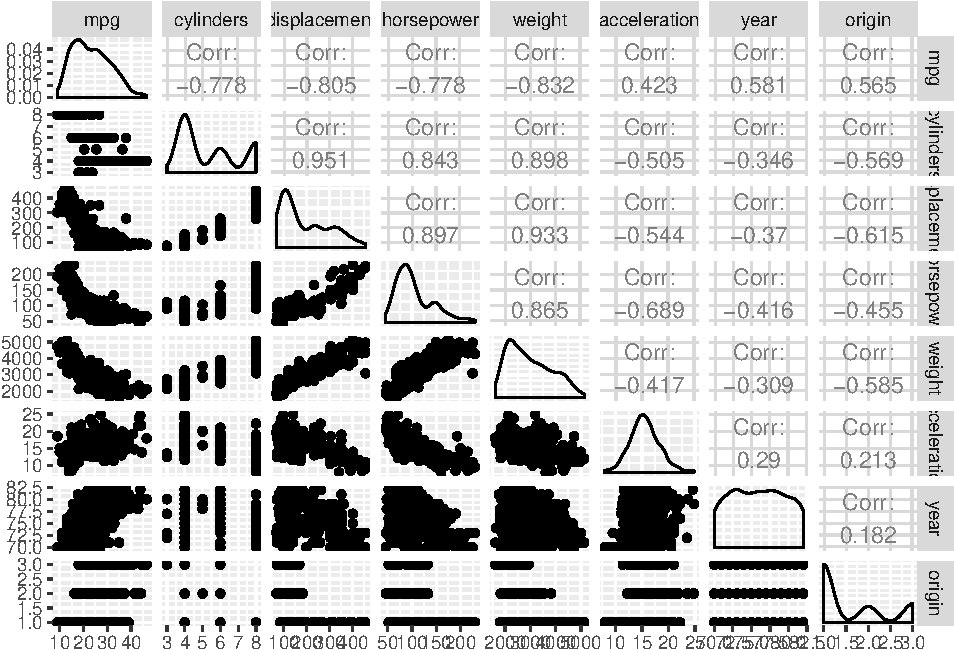
\includegraphics{9SVM_files/figure-beamer/unnamed-chunk-3-1.pdf}

\end{frame}

\begin{frame}[fragile]

\begin{Shaded}
\begin{Highlighting}[]
\KeywordTok{summary}\NormalTok{(svmfit_linear1)}
\end{Highlighting}
\end{Shaded}

\begin{verbatim}
## 
## Call:
## svm(formula = y ~ ., data = train2, kernel = "linear", cost = 1, 
##     scale = FALSE)
## 
## 
## Parameters:
##    SVM-Type:  C-classification 
##  SVM-Kernel:  linear 
##        cost:  1 
## 
## Number of Support Vectors:  56
## 
##  ( 28 28 )
## 
## 
## Number of Classes:  2 
## 
## Levels: 
##  -1 1
\end{verbatim}

\begin{Shaded}
\begin{Highlighting}[]
\NormalTok{svmfit_linear1}\OperatorTok{$}\NormalTok{index  }\CommentTok{#support vectors id in data set}
\end{Highlighting}
\end{Shaded}

\begin{verbatim}
##  [1]  1  2  4  6  9 10 16 21 26 27 28 40 44 53 55 57 58 65 67 72 76 77 80
## [24] 81 87 91 92 98  5  8 11 13 18 19 20 23 24 25 34 36 39 41 42 47 48 59
## [47] 61 62 70 71 75 78 88 93 95 96
\end{verbatim}

\normalsize

\end{frame}

\begin{frame}

\textbf{Observations}

\begin{itemize}
\tightlist
\item
  Remark that the \(x_1\) is plotted on the vertical axis, and the the
  implementation of the plotting function is made in a way that the
  linear boundary looks jagged.
\item
  The crosses in the plot indicate the support vectors. With \(cost=1\),
  we have 56 support vectors, 28 in each class.
\item
  All other observations are shown as circles.
\end{itemize}

\end{frame}

\begin{frame}[fragile]

Next, we set \(cost=100\): \footnotesize

\begin{Shaded}
\begin{Highlighting}[]
\NormalTok{svmfit_linear2 =}\StringTok{ }\KeywordTok{svm}\NormalTok{(y }\OperatorTok{~}\StringTok{ }\NormalTok{., }\DataTypeTok{data =}\NormalTok{ train2, }\DataTypeTok{kernel =} \StringTok{"linear"}\NormalTok{, }\DataTypeTok{cost =} \DecValTok{100}\NormalTok{, }
    \DataTypeTok{scale =} \OtherTok{FALSE}\NormalTok{)}
\KeywordTok{plot}\NormalTok{(svmfit_linear2, train2, }\DataTypeTok{col =} \KeywordTok{c}\NormalTok{(}\StringTok{"lightcoral"}\NormalTok{, }\StringTok{"lightgreen"}\NormalTok{))}
\end{Highlighting}
\end{Shaded}

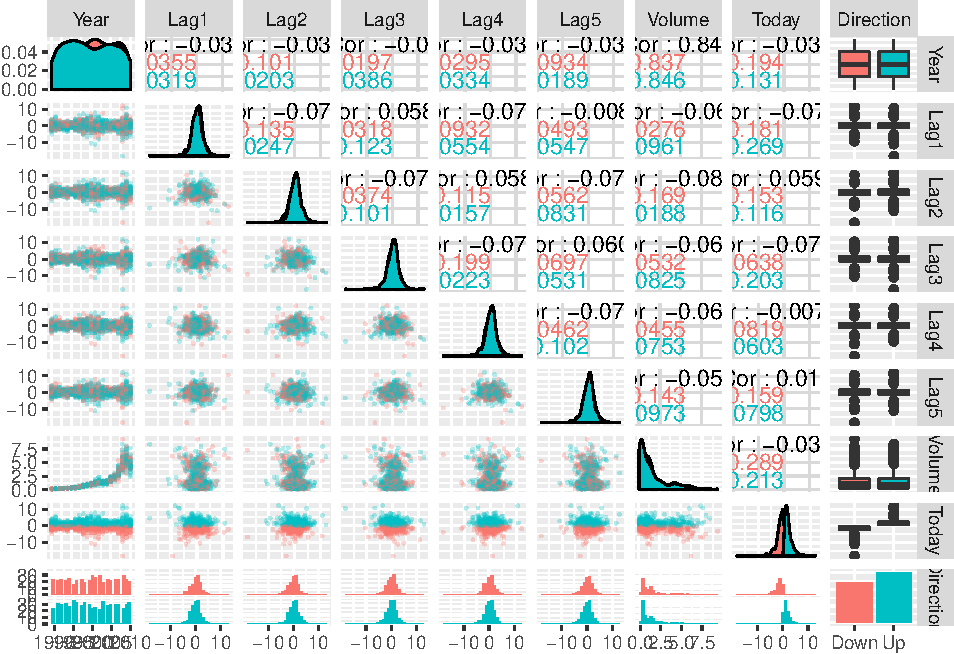
\includegraphics{9SVM_files/figure-beamer/unnamed-chunk-5-1.pdf}

\end{frame}

\begin{frame}[fragile]

\begin{Shaded}
\begin{Highlighting}[]
\KeywordTok{summary}\NormalTok{(svmfit_linear2)}
\end{Highlighting}
\end{Shaded}

\begin{verbatim}
## 
## Call:
## svm(formula = y ~ ., data = train2, kernel = "linear", cost = 100, 
##     scale = FALSE)
## 
## 
## Parameters:
##    SVM-Type:  C-classification 
##  SVM-Kernel:  linear 
##        cost:  100 
## 
## Number of Support Vectors:  31
## 
##  ( 15 16 )
## 
## 
## Number of Classes:  2 
## 
## Levels: 
##  -1 1
\end{verbatim}

\normalsize

\end{frame}

\begin{frame}[fragile]

With \(cost=100\) we have 31 support vectors, i.e the width of the
margin is decreased.

How do we find an optimal \(cost\) parameter? By using the \emph{tune()}
function we can perform ten-fold cross-validation and find the
cost-parameter that gives the lowest cross-validation error:

\footnotesize

\begin{Shaded}
\begin{Highlighting}[]
\KeywordTok{set.seed}\NormalTok{(}\DecValTok{1}\NormalTok{)}
\NormalTok{CV_linear =}\StringTok{ }\KeywordTok{tune}\NormalTok{(svm, y }\OperatorTok{~}\StringTok{ }\NormalTok{., }\DataTypeTok{data =}\NormalTok{ train2, }\DataTypeTok{kernel =} \StringTok{"linear"}\NormalTok{, }\DataTypeTok{ranges =} \KeywordTok{list}\NormalTok{(}\DataTypeTok{cost =} \KeywordTok{c}\NormalTok{(}\FloatTok{0.001}\NormalTok{, }
    \FloatTok{0.01}\NormalTok{, }\FloatTok{0.1}\NormalTok{, }\DecValTok{1}\NormalTok{, }\DecValTok{5}\NormalTok{, }\DecValTok{10}\NormalTok{, }\DecValTok{100}\NormalTok{)))}
\KeywordTok{summary}\NormalTok{(CV_linear)}
\end{Highlighting}
\end{Shaded}

\begin{verbatim}
## 
## Parameter tuning of 'svm':
## 
## - sampling method: 10-fold cross validation 
## 
## - best parameters:
##  cost
##     5
## 
## - best performance: 0.14 
## 
## - Detailed performance results:
##    cost error dispersion
## 1 1e-03  0.45 0.10801234
## 2 1e-02  0.23 0.12516656
## 3 1e-01  0.16 0.11737878
## 4 1e+00  0.15 0.10801234
## 5 5e+00  0.14 0.10749677
## 6 1e+01  0.15 0.09718253
## 7 1e+02  0.15 0.09718253
\end{verbatim}

\normalsize

\end{frame}

\begin{frame}[fragile]

According to the \emph{tune()} function we should set the cost parameter
to 0.1. The function also stores the best model obtained and we can
access it as follows:

\begin{Shaded}
\begin{Highlighting}[]
\NormalTok{bestmod_linear =}\StringTok{ }\NormalTok{CV_linear}\OperatorTok{$}\NormalTok{best.model}
\end{Highlighting}
\end{Shaded}

Next, we want to predict the class label of the seeds in the test set.
We use the \texttt{predict} function and make a confusion table:

\begin{Shaded}
\begin{Highlighting}[]
\NormalTok{ypred_linear =}\StringTok{ }\KeywordTok{predict}\NormalTok{(bestmod_linear, test2)}
\KeywordTok{table}\NormalTok{(}\DataTypeTok{predict =}\NormalTok{ ypred_linear, }\DataTypeTok{truth =}\NormalTok{ test2[, }\DecValTok{3}\NormalTok{])}
\end{Highlighting}
\end{Shaded}

\begin{verbatim}
##        truth
## predict -1  1
##      -1  8  0
##      1   2 10
\end{verbatim}

\end{frame}

\begin{frame}[fragile]

\footnotesize

\begin{Shaded}
\begin{Highlighting}[]
\KeywordTok{par}\NormalTok{(}\DataTypeTok{mfrow =} \KeywordTok{c}\NormalTok{(}\DecValTok{1}\NormalTok{, }\DecValTok{2}\NormalTok{))}
\KeywordTok{par}\NormalTok{(}\DataTypeTok{pty =} \StringTok{"s"}\NormalTok{)}
\KeywordTok{plot}\NormalTok{(}\OtherTok{NA}\NormalTok{, }\DataTypeTok{xlab =} \StringTok{"x1"}\NormalTok{, }\DataTypeTok{ylab =} \StringTok{"x2"}\NormalTok{, }\DataTypeTok{xlim =} \KeywordTok{c}\NormalTok{(}\DecValTok{0}\NormalTok{, }\DecValTok{1}\NormalTok{), }\DataTypeTok{ylim =} \KeywordTok{c}\NormalTok{(}\DecValTok{0}\NormalTok{, }\DecValTok{1}\NormalTok{))}
\KeywordTok{title}\NormalTok{(}\StringTok{"True class"}\NormalTok{)}
\KeywordTok{points}\NormalTok{(seeds2[seeds2[, }\DecValTok{3}\NormalTok{] }\OperatorTok{==}\StringTok{ }\DecValTok{-1}\NormalTok{, }\DecValTok{1}\OperatorTok{:}\DecValTok{2}\NormalTok{], }\DataTypeTok{pch =} \DecValTok{19}\NormalTok{, }\DataTypeTok{col =} \StringTok{"lightcoral"}\NormalTok{, }
    \DataTypeTok{cex =} \FloatTok{0.9}\NormalTok{)}
\KeywordTok{points}\NormalTok{(seeds2[seeds2[, }\DecValTok{3}\NormalTok{] }\OperatorTok{==}\StringTok{ }\DecValTok{1}\NormalTok{, }\DecValTok{1}\OperatorTok{:}\DecValTok{2}\NormalTok{], }\DataTypeTok{pch =} \DecValTok{19}\NormalTok{, }\DataTypeTok{col =} \StringTok{"darkseagreen"}\NormalTok{, }
    \DataTypeTok{cex =} \FloatTok{0.9}\NormalTok{)}
\KeywordTok{points}\NormalTok{(seeds2[}\KeywordTok{which}\NormalTok{(ypred_linear }\OperatorTok{!=}\StringTok{ }\NormalTok{seeds2[, }\DecValTok{3}\NormalTok{]), }\DecValTok{1}\OperatorTok{:}\DecValTok{2}\NormalTok{], }\DataTypeTok{pch =} \DecValTok{21}\NormalTok{)  }\CommentTok{#Mark misclassification.}

\KeywordTok{plot}\NormalTok{(}\OtherTok{NA}\NormalTok{, }\DataTypeTok{xlab =} \StringTok{"x1"}\NormalTok{, }\DataTypeTok{ylab =} \StringTok{"x2"}\NormalTok{, }\DataTypeTok{xlim =} \KeywordTok{c}\NormalTok{(}\DecValTok{0}\NormalTok{, }\DecValTok{1}\NormalTok{), }\DataTypeTok{ylim =} \KeywordTok{c}\NormalTok{(}\DecValTok{0}\NormalTok{, }\DecValTok{1}\NormalTok{))}
\KeywordTok{title}\NormalTok{(}\StringTok{"Predicted class"}\NormalTok{)}
\KeywordTok{points}\NormalTok{(seeds2[ypred_linear }\OperatorTok{==}\StringTok{ }\DecValTok{-1}\NormalTok{, }\DecValTok{1}\OperatorTok{:}\DecValTok{2}\NormalTok{], }\DataTypeTok{pch =} \DecValTok{19}\NormalTok{, }\DataTypeTok{col =} \StringTok{"lightcoral"}\NormalTok{, }
    \DataTypeTok{cex =} \FloatTok{0.9}\NormalTok{)}
\KeywordTok{points}\NormalTok{(seeds2[ypred_linear }\OperatorTok{==}\StringTok{ }\DecValTok{1}\NormalTok{, }\DecValTok{1}\OperatorTok{:}\DecValTok{2}\NormalTok{], }\DataTypeTok{pch =} \DecValTok{19}\NormalTok{, }\DataTypeTok{col =} \StringTok{"darkseagreen"}\NormalTok{, }
    \DataTypeTok{cex =} \FloatTok{0.9}\NormalTok{)}
\KeywordTok{points}\NormalTok{(seeds2[}\KeywordTok{which}\NormalTok{(ypred_linear }\OperatorTok{!=}\StringTok{ }\NormalTok{seeds2[, }\DecValTok{3}\NormalTok{]), }\DecValTok{1}\OperatorTok{:}\DecValTok{2}\NormalTok{], }\DataTypeTok{pch =} \DecValTok{21}\NormalTok{)  }\CommentTok{#Mark misclassification.}
\end{Highlighting}
\end{Shaded}

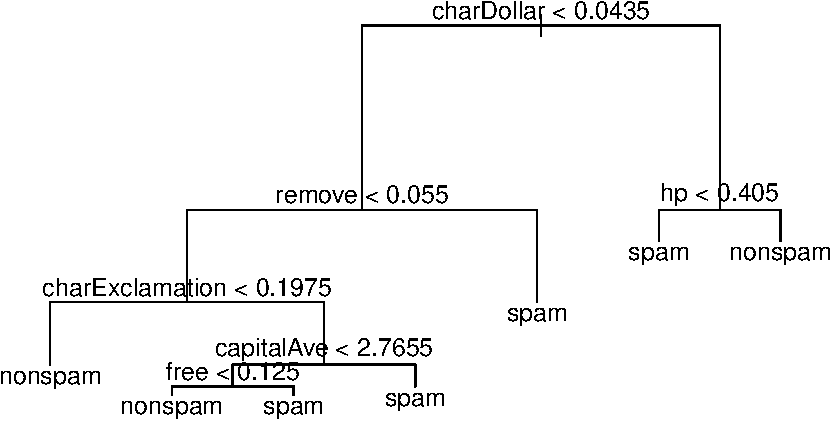
\includegraphics{9SVM_files/figure-beamer/unnamed-chunk-10-1.pdf}

\normalsize

\end{frame}

\begin{frame}[fragile]

In this case three of the test observations are misclassified: These
three observations are marked with a black circle in the plot, and we
observe that they lie on the border between the green and the orange
points which is reasonable: The test observations located on the border
between green and orange are hardest to predict.

Missing: the \texttt{svm} function is not (directly) outputting the
equation for the class boundary, and not the value for the width of the
margin. Want to see how to find this? See the recommended exercises.

\end{frame}

\begin{frame}{Support Vector Machines}

For some datasets a non-linear decicion boundary between the classes is
more suitable than a linear decision boundary. In such cases you can use
a \textbf{Support Vector Machine} (SVM). This is an extension of the
support vector classifier.

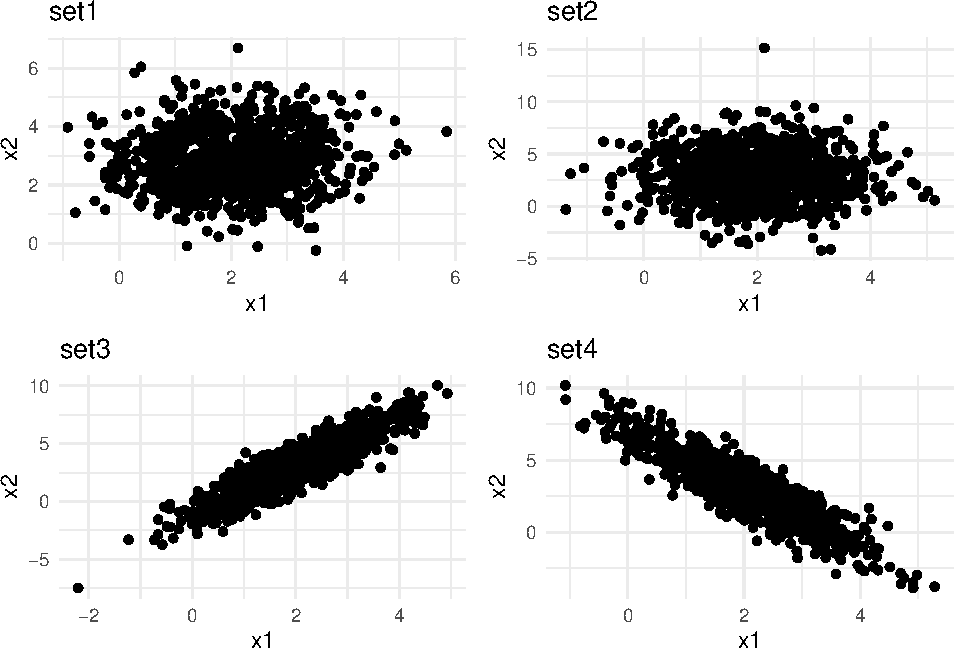
\includegraphics{9SVM_files/figure-beamer/unnamed-chunk-11-1.pdf}

\end{frame}

\begin{frame}

\begin{block}{Expanding the feature space}

We saw in Module 7 that in regression we could fit non-linear curves by
using a polynomial basis - adding polynomials of different order as
covariates. This was a linear regression in the transformed variables,
but non-linear in the original variables. Maybe we may add many such
extra features and find a nice linear boundary in that high-dimensional
space?

Efron and Hastie (2016) (page 377): \emph{If \(n \le p+1\) we can always
find a separating hyperplane, unless there are exact features ties
across the class barrier.} (Two observations with equal covariate
vector, but different classes.)

\end{block}

\end{frame}

\begin{frame}

\includegraphics{../../ISLR/Figures/Chapter9/9.9.png}

Left: expanding feature space to include cubic polynomials
(\(x_1,x_2,x_1x_2,x_1^2,x_2^2,x_1^2x_2,x_1x_2^2x_1^3,x_2^3\), 9
parameters to estimate in addition to intercept), and also observe the
margins. (Right: radial basis function kernel - wait a bit.)

Next: replace polynomials with \emph{kernels} for elegance and
computational issues.

\end{frame}

\begin{frame}

\begin{block}{Inner products}

We have not focused on how to solve the optimisation problem of finding
the support vector classifier hyperplane, because this is outside the
scope of this course.

Remember that we classify a new observation \({\boldsymbol x}^*\) by
first calculating a numerical value for the estimated
\(f({\boldsymbol x}^*)\) and then if \(f({\boldsymbol x}^*)<0\) classify
as \(-1\) and if \(f({\boldsymbol x}^*)>0\) classify as \(1\).

It can be \emph{shown} (using optimization theory) that the solution to
the support vector classifier problem at a new observation
\({\boldsymbol x}^*\), can be expressed as \[
f({\boldsymbol x}^*)=\beta_0 + \sum_{i=1}^n \alpha_i \langle {\boldsymbol x}^*,{\boldsymbol x}_i \rangle
\] where \(\alpha_i\) is some parameter and \(i=1,...,n\).

\end{block}

\end{frame}

\begin{frame}

A term of the form
\(\langle {\boldsymbol x}_i, {\boldsymbol x}_{i'} \rangle\) denotes the
inner product between two observations \(i\) and \(i'\) and is defined
as: \[
\langle {\boldsymbol x}_i , {\boldsymbol x}_{i'}\rangle =\sum_{j=1}^p x_{ij} x_{i' j}.
\] This means that we need (in addition to the intercept) to estimate
\(n\) parameters (\(\alpha_i\)s) instead of \(p\) (\(\beta_j\)s) (and
for our expanded feature space then \(p\) might be larger than \(n\)).
(For the interested reader: See Eq. 19.22 and 19.23 of Efron and Hastie
(2016).)

\end{frame}

\begin{frame}

Further, it then turns out that to estimate the parameters
\(\beta_0,\alpha_1,...,\alpha_n\) this can be based on the
\({n choose 2}\) inner products
\(\langle {\boldsymbol x}_i,{\boldsymbol x}_i' \rangle\) between all
pair of training observations (the class of the training observations is
also included).

Also, \(\alpha_i=0\) for the observations \(i\) that are \emph{not} the
support vectors. Remark: we could alternatively say that
\(\alpha_i \neq 0\) define the support vectors.

\end{frame}

\begin{frame}

Thus, we only need the inner product between the new observation and the
observations corresponding to support vectors to classify a new
observation, and

\[
f({\boldsymbol x})=\beta_0 + \sum_{i \in \mathcal{S}} \alpha_i \langle {\boldsymbol x}, {\boldsymbol x}_i\rangle,
\] where \(\mathcal{S}\) contains the indices of the support points. So,
we have sparsity in the observations (but not in the predictors).

\end{frame}

\begin{frame}

\textbf{Q:} Find the support vectors

\includegraphics{../../ISLR/Figures/Chapter9/9.6.png}

Observe: we need all observations (both \(x\) and \(y\) values) to
decide on which observations are the support vectors.

\end{frame}

\begin{frame}

\begin{block}{Kernels}

(we now use \(x\) to denote a new observation)

The next step is now to \emph{replace the inner product}
\(\langle {\boldsymbol x}, {\boldsymbol x}_i\rangle\) with a function
\(K({\boldsymbol x}_i,{\boldsymbol x}_{i'})\) referred to as the
\textbf{kernel}: \[
f({\boldsymbol x})=\beta_0 + \sum_{i \in \mathcal{S}} \alpha_i K({\boldsymbol x},{\boldsymbol x}_i).
\] For the linear case (which is what we have considered so far), the
kernel is simply the inner product
\(K({\boldsymbol x}_i,{\boldsymbol x}_i')=\sum_{j=1}^p x_{ij}x_{i'j}\).

The two arguments to the kernel are two \(p\)-vectors.

If we want a more flexible decision boundary we could instead use a
\textbf{polynomial kernel}. This polynomial kernel of degree \(d>1\) is
given by: \[
K({\boldsymbol x}_i,{\boldsymbol x}_i')=(1+\sum_{j1}^p x_{ij} x_{i'j})^d.
\] (This kernel is not so much used in practice, but is popular for
proofs.)

\end{block}

\end{frame}

\begin{frame}

Using these kernels our solution for the class boundary can be written
of the form

\[f({\boldsymbol x})=\beta_0 +\sum_{i\in \cal{S}} \alpha_i K({\boldsymbol x},{\boldsymbol x}_i)\]

The nice thing here is that we only need to calculate the kernels, not
the basis functions (what we in Module 7 did as extra columns of the
design matrix).

\end{frame}

\begin{frame}

A very popular choice is the radial kernel, \[
K({\boldsymbol x}_i,{\boldsymbol x}_i')=\exp(-\gamma \sum_{j=1}^p (x_{ij}-x_{i'j})^2),
\] where \(\gamma\) is a positive constant (a tuning parameter).

Observe the connection to a multivariate normal density, where
\(\gamma \propto 1/\sigma^2\) (\(\sigma^2\) variance in normal
distribution). If \(\gamma\) is small (similar to large variance in the
normal distribution) the decision boundaries are smoother than for
larger \(\gamma\).

It turns out that this computes the inner product in a very high
(infinite) dimensional feature space. But, this does not give
overfitting because some of the dimensions are ``squashed down'' (but we
have the parameter \(\gamma\) and the budget parameter that we have to
decide on).

The radial kernel is convinient if we want a circular decision boundary,
and \(\gamma\) and our budget can be chosen by cross-validation.

Remark: the mathematics behind this is based on \emph{reproducing-kernel
Hilbert spaces} (see page 384 of Efron and Hastie (2016) for a glimpse
of the theory).

\end{frame}

\begin{frame}

Study Figures 19.5 and 19.6 (page 383) in Efron and Hastie (2016) to see
how the radial kernel can make smooth functions.

\href{https://web.stanford.edu/~hastie/CASI_files/PDF/casi.pdf}{Computer
Age Statistical Inference}

\end{frame}

\begin{frame}

\begin{block}{Kernels and our optimization}

We now merge our optimization problem (from our support vector
classifier) with our kernel representation \(f({\boldsymbol x})\) to get
the Support Vector Machine (SVM).

\[\mathrm{maximize}_{\beta_0,\alpha_1,...,\alpha_n,\epsilon_1,...,\epsilon_n,} \quad M \]
\[y_i(f({\boldsymbol x}_i))\geq M(1-\epsilon_i) \quad  \forall i=1,...,n.\]
\[\epsilon_i\geq 0, \quad \sum_{i=1}^n \epsilon_i \leq C.\]

where
\[f({\boldsymbol x}_i)=\beta_0 +\sum_{l\in \cal{S}} \alpha_l K({\boldsymbol x}_i,{\boldsymbol x}_l)\]

\end{block}

\end{frame}

\begin{frame}

\begin{block}{Tuning parameter example}

Heart data - predict heart disease from \(p=13\) predictors.

Training errors as ROC and AUC.

\includegraphics{../../ISLR/Figures/Chapter9/9.10.png}

\end{block}

\end{frame}

\begin{frame}

Heart data - test error.

\includegraphics{../../ISLR/Figures/Chapter9/9.11.png}

\end{frame}

\begin{frame}[fragile]

\begin{block}{Example: forest 3}

To illustrate the SVM we use the third training dataset (forest3) and
the third test set (seeds3). We use the \texttt{svm} function as before.
However, we now set
\texttt{kernel=\textquotesingle{}radial\textquotesingle{}} as we want a
non-linear decision boundary:

\end{block}

\end{frame}

\begin{frame}[fragile]

\footnotesize

\begin{Shaded}
\begin{Highlighting}[]
\KeywordTok{library}\NormalTok{(e1071)}
\NormalTok{forest3 =}\StringTok{ }\KeywordTok{read.table}\NormalTok{(}\DataTypeTok{file =} \StringTok{"forest3.txt"}\NormalTok{)}
\NormalTok{seeds3 =}\StringTok{ }\KeywordTok{read.table}\NormalTok{(}\DataTypeTok{file =} \StringTok{"seeds3.txt"}\NormalTok{)}
\NormalTok{train3 =}\StringTok{ }\KeywordTok{data.frame}\NormalTok{(}\DataTypeTok{x =}\NormalTok{ forest3[, }\DecValTok{1}\OperatorTok{:}\DecValTok{2}\NormalTok{], }\DataTypeTok{y =} \KeywordTok{as.factor}\NormalTok{(forest3[, }\DecValTok{3}\NormalTok{]))}
\NormalTok{test3 =}\StringTok{ }\KeywordTok{data.frame}\NormalTok{(}\DataTypeTok{x =}\NormalTok{ seeds3[, }\DecValTok{1}\OperatorTok{:}\DecValTok{2}\NormalTok{], }\DataTypeTok{y =} \KeywordTok{as.factor}\NormalTok{(seeds3[, }\DecValTok{3}\NormalTok{]))}
\end{Highlighting}
\end{Shaded}

\end{frame}

\begin{frame}[fragile]

\begin{Shaded}
\begin{Highlighting}[]
\NormalTok{svmfit_kernel1 =}\StringTok{ }\KeywordTok{svm}\NormalTok{(y }\OperatorTok{~}\StringTok{ }\NormalTok{., }\DataTypeTok{data =}\NormalTok{ train3, }\DataTypeTok{kernel =} \StringTok{"radial"}\NormalTok{, }\DataTypeTok{gamma =} \DecValTok{1}\NormalTok{, }
    \DataTypeTok{cost =} \DecValTok{10}\NormalTok{, }\DataTypeTok{scale =} \OtherTok{FALSE}\NormalTok{)}
\KeywordTok{plot}\NormalTok{(svmfit_kernel1, train3, }\DataTypeTok{col =} \KeywordTok{c}\NormalTok{(}\StringTok{"lightcoral"}\NormalTok{, }\StringTok{"lightgreen"}\NormalTok{))}
\end{Highlighting}
\end{Shaded}

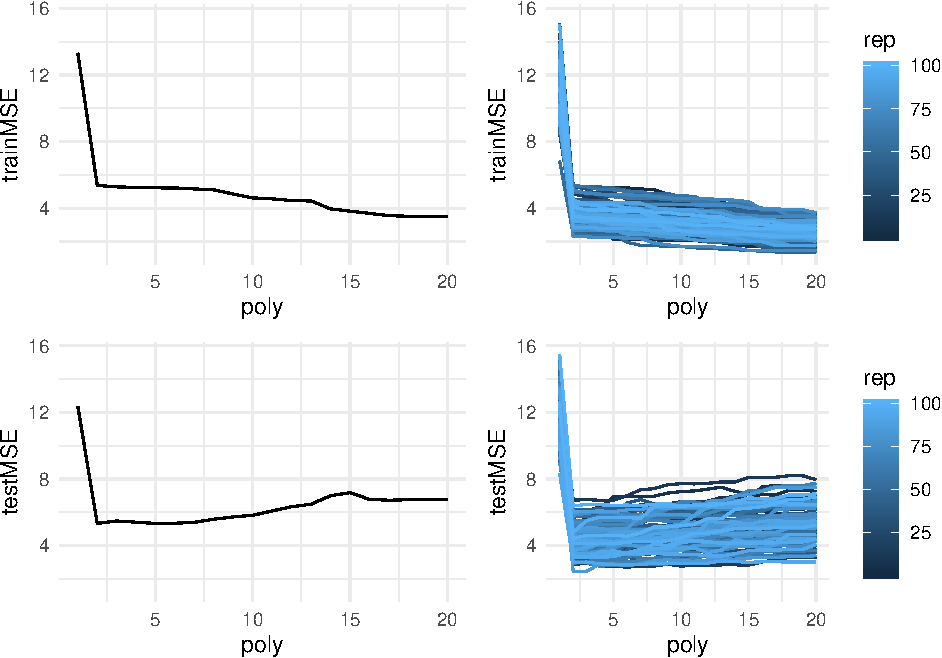
\includegraphics{9SVM_files/figure-beamer/unnamed-chunk-13-1.pdf}

\begin{Shaded}
\begin{Highlighting}[]
\KeywordTok{summary}\NormalTok{(svmfit_kernel1)}
\end{Highlighting}
\end{Shaded}

\begin{verbatim}
## 
## Call:
## svm(formula = y ~ ., data = train3, kernel = "radial", gamma = 1, 
##     cost = 10, scale = FALSE)
## 
## 
## Parameters:
##    SVM-Type:  C-classification 
##  SVM-Kernel:  radial 
##        cost:  10 
## 
## Number of Support Vectors:  31
## 
##  ( 16 15 )
## 
## 
## Number of Classes:  2 
## 
## Levels: 
##  -1 1
\end{verbatim}

\normalsize

\end{frame}

\begin{frame}[fragile]

We could also try with a polynomial kernel with degree 4 as follows:

\footnotesize

\begin{Shaded}
\begin{Highlighting}[]
\NormalTok{svmfit_kernel2 =}\StringTok{ }\KeywordTok{svm}\NormalTok{(y }\OperatorTok{~}\StringTok{ }\NormalTok{., }\DataTypeTok{data =}\NormalTok{ train3, }\DataTypeTok{kernel =} \StringTok{"polynomial"}\NormalTok{, }
    \DataTypeTok{degree =} \DecValTok{4}\NormalTok{, }\DataTypeTok{cost =} \FloatTok{1e+05}\NormalTok{, }\DataTypeTok{scale =} \OtherTok{FALSE}\NormalTok{)}
\KeywordTok{plot}\NormalTok{(svmfit_kernel2, train3, }\DataTypeTok{col =} \KeywordTok{c}\NormalTok{(}\StringTok{"lightcoral"}\NormalTok{, }\StringTok{"lightgreen"}\NormalTok{))}
\end{Highlighting}
\end{Shaded}

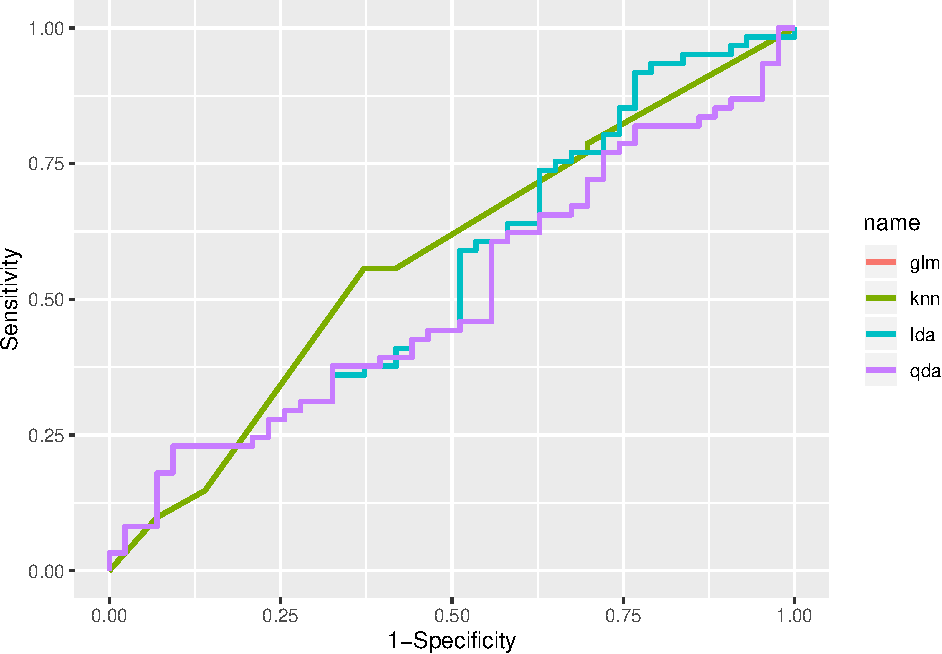
\includegraphics{9SVM_files/figure-beamer/unnamed-chunk-14-1.pdf}

\end{frame}

\begin{frame}[fragile]

\begin{Shaded}
\begin{Highlighting}[]
\KeywordTok{summary}\NormalTok{(svmfit_kernel2)}
\end{Highlighting}
\end{Shaded}

\begin{verbatim}
## 
## Call:
## svm(formula = y ~ ., data = train3, kernel = "polynomial", degree = 4, 
##     cost = 1e+05, scale = FALSE)
## 
## 
## Parameters:
##    SVM-Type:  C-classification 
##  SVM-Kernel:  polynomial 
##        cost:  1e+05 
##      degree:  4 
##      coef.0:  0 
## 
## Number of Support Vectors:  40
## 
##  ( 21 19 )
## 
## 
## Number of Classes:  2 
## 
## Levels: 
##  -1 1
\end{verbatim}

\normalsize

\end{frame}

\begin{frame}[fragile]

For this dataset a radial kernel is a natural choice: A circular
decision boundary seems like a good idea. Thus, we proceed with
\texttt{kernel=\textquotesingle{}radial\textquotesingle{}}, and use the
\texttt{tune()} function to find the optimal tuning parameter \(C\):

\footnotesize

\begin{Shaded}
\begin{Highlighting}[]
\KeywordTok{set.seed}\NormalTok{(}\DecValTok{1}\NormalTok{)}
\NormalTok{CV_kernel =}\StringTok{ }\KeywordTok{tune}\NormalTok{(svm, y }\OperatorTok{~}\StringTok{ }\NormalTok{., }\DataTypeTok{data =}\NormalTok{ train3, }\DataTypeTok{kernel =} \StringTok{"radial"}\NormalTok{, }\DataTypeTok{gamma =} \DecValTok{1}\NormalTok{, }
    \DataTypeTok{ranges =} \KeywordTok{list}\NormalTok{(}\DataTypeTok{cost =} \KeywordTok{c}\NormalTok{(}\FloatTok{0.001}\NormalTok{, }\FloatTok{0.01}\NormalTok{, }\FloatTok{0.1}\NormalTok{, }\DecValTok{1}\NormalTok{, }\DecValTok{5}\NormalTok{, }\DecValTok{10}\NormalTok{, }\DecValTok{100}\NormalTok{)))}
\KeywordTok{summary}\NormalTok{(CV_kernel)}
\end{Highlighting}
\end{Shaded}

\begin{verbatim}
## 
## Parameter tuning of 'svm':
## 
## - sampling method: 10-fold cross validation 
## 
## - best parameters:
##  cost
##   100
## 
## - best performance: 0.1089286 
## 
## - Detailed performance results:
##    cost     error dispersion
## 1 1e-03 0.2732143  0.1472658
## 2 1e-02 0.2732143  0.1472658
## 3 1e-01 0.2732143  0.1472658
## 4 1e+00 0.1500000  0.1315463
## 5 5e+00 0.1357143  0.1226248
## 6 1e+01 0.1214286  0.1298110
## 7 1e+02 0.1089286  0.1066291
\end{verbatim}

\normalsize

\end{frame}

\begin{frame}[fragile]

The optimal \(C\) is 10. Next, we predict the class label of the seeds
in the test set with a model with C=10, make a confusion table and plot
the results:

\begin{Shaded}
\begin{Highlighting}[]
\NormalTok{bestmod_kernel =}\StringTok{ }\NormalTok{CV_kernel}\OperatorTok{$}\NormalTok{best.model}
\NormalTok{ypred_kernel =}\StringTok{ }\KeywordTok{predict}\NormalTok{(bestmod_kernel, test3)}
\end{Highlighting}
\end{Shaded}

\end{frame}

\begin{frame}[fragile]

\begin{Shaded}
\begin{Highlighting}[]
\KeywordTok{par}\NormalTok{(}\DataTypeTok{mfrow =} \KeywordTok{c}\NormalTok{(}\DecValTok{1}\NormalTok{, }\DecValTok{3}\NormalTok{))}
\KeywordTok{par}\NormalTok{(}\DataTypeTok{pty =} \StringTok{"s"}\NormalTok{)}
\KeywordTok{plot}\NormalTok{(}\OtherTok{NA}\NormalTok{, }\DataTypeTok{xlab =} \StringTok{"x1"}\NormalTok{, }\DataTypeTok{ylab =} \StringTok{"x2"}\NormalTok{, }\DataTypeTok{xlim =} \KeywordTok{c}\NormalTok{(}\DecValTok{0}\NormalTok{, }\DecValTok{1}\NormalTok{), }\DataTypeTok{ylim =} \KeywordTok{c}\NormalTok{(}\DecValTok{0}\NormalTok{, }\DecValTok{1}\NormalTok{))}
\KeywordTok{title}\NormalTok{(}\StringTok{"True class"}\NormalTok{)}
\KeywordTok{points}\NormalTok{(seeds3[seeds3[, }\DecValTok{3}\NormalTok{] }\OperatorTok{==}\StringTok{ }\DecValTok{-1}\NormalTok{, }\DecValTok{1}\OperatorTok{:}\DecValTok{2}\NormalTok{], }\DataTypeTok{pch =} \DecValTok{19}\NormalTok{, }\DataTypeTok{col =} \StringTok{"lightcoral"}\NormalTok{, }
    \DataTypeTok{cex =} \FloatTok{0.9}\NormalTok{)}
\KeywordTok{points}\NormalTok{(seeds3[seeds3[, }\DecValTok{3}\NormalTok{] }\OperatorTok{==}\StringTok{ }\DecValTok{1}\NormalTok{, }\DecValTok{1}\OperatorTok{:}\DecValTok{2}\NormalTok{], }\DataTypeTok{pch =} \DecValTok{19}\NormalTok{, }\DataTypeTok{col =} \StringTok{"darkseagreen"}\NormalTok{, }
    \DataTypeTok{cex =} \FloatTok{0.9}\NormalTok{)}
\KeywordTok{points}\NormalTok{(seeds3[}\KeywordTok{which}\NormalTok{(ypred_kernel }\OperatorTok{!=}\StringTok{ }\NormalTok{seeds3[, }\DecValTok{3}\NormalTok{]), }\DecValTok{1}\OperatorTok{:}\DecValTok{2}\NormalTok{], }\DataTypeTok{pch =} \DecValTok{21}\NormalTok{)  }\CommentTok{#Mark misclassification.}
\end{Highlighting}
\end{Shaded}

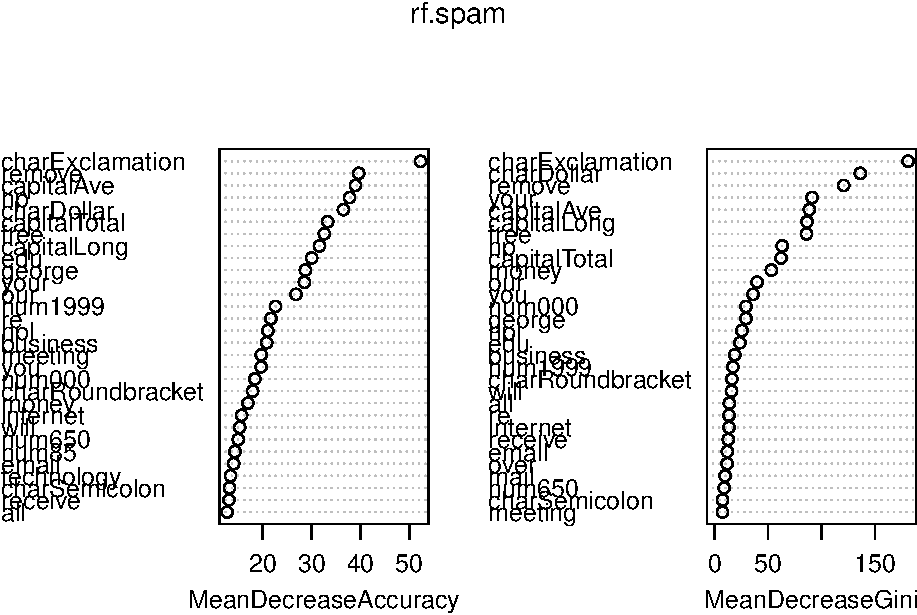
\includegraphics{9SVM_files/figure-beamer/unnamed-chunk-18-1.pdf}

\end{frame}

\begin{frame}[fragile]

\begin{Shaded}
\begin{Highlighting}[]
\KeywordTok{plot}\NormalTok{(}\OtherTok{NA}\NormalTok{, }\DataTypeTok{xlab =} \StringTok{"x1"}\NormalTok{, }\DataTypeTok{ylab =} \StringTok{"x2"}\NormalTok{, }\DataTypeTok{xlim =} \KeywordTok{c}\NormalTok{(}\DecValTok{0}\NormalTok{, }\DecValTok{1}\NormalTok{), }\DataTypeTok{ylim =} \KeywordTok{c}\NormalTok{(}\DecValTok{0}\NormalTok{, }\DecValTok{1}\NormalTok{))}
\KeywordTok{title}\NormalTok{(}\StringTok{"Predicted class"}\NormalTok{)}
\KeywordTok{points}\NormalTok{(seeds3[ypred_kernel }\OperatorTok{==}\StringTok{ }\DecValTok{-1}\NormalTok{, }\DecValTok{1}\OperatorTok{:}\DecValTok{2}\NormalTok{], }\DataTypeTok{pch =} \DecValTok{19}\NormalTok{, }\DataTypeTok{col =} \StringTok{"lightcoral"}\NormalTok{, }
    \DataTypeTok{cex =} \FloatTok{0.9}\NormalTok{)}
\KeywordTok{points}\NormalTok{(seeds3[ypred_kernel }\OperatorTok{==}\StringTok{ }\DecValTok{1}\NormalTok{, }\DecValTok{1}\OperatorTok{:}\DecValTok{2}\NormalTok{], }\DataTypeTok{pch =} \DecValTok{19}\NormalTok{, }\DataTypeTok{col =} \StringTok{"darkseagreen"}\NormalTok{, }
    \DataTypeTok{cex =} \FloatTok{0.9}\NormalTok{)}
\KeywordTok{points}\NormalTok{(seeds3[}\KeywordTok{which}\NormalTok{(ypred_kernel }\OperatorTok{!=}\StringTok{ }\NormalTok{seeds3[, }\DecValTok{3}\NormalTok{]), }\DecValTok{1}\OperatorTok{:}\DecValTok{2}\NormalTok{], }\DataTypeTok{pch =} \DecValTok{21}\NormalTok{)  }\CommentTok{#Mark misclassification.}
\end{Highlighting}
\end{Shaded}

\includegraphics{9SVM_files/figure-beamer/unnamed-chunk-19-1.pdf}

\begin{Shaded}
\begin{Highlighting}[]
\KeywordTok{table}\NormalTok{(}\DataTypeTok{predict =}\NormalTok{ ypred_kernel, }\DataTypeTok{truth =}\NormalTok{ test3[, }\DecValTok{3}\NormalTok{])}
\end{Highlighting}
\end{Shaded}

\begin{verbatim}
##        truth
## predict -1 1
##      -1  9 0
##      1   1 5
\end{verbatim}

Only one seed is misclassified.

\end{frame}

\begin{frame}[fragile]{Extensions}

\begin{block}{More than two classes}

What if we have \(k\) classes?

\begin{itemize}
\tightlist
\item
  OVA: one-versus-all. Fit \(k\) different two-class SVMs
  \(f_k({\boldsymbol x})\) where one class is compared to all other
  classes. Classify a test observation to the class where
  \(f_k({\boldsymbol x}^*)\) is largest.
\item
  OVO: one-versus-one. \texttt{libsvm} uses this approach, in which
  \(k(k-1)/2\) binary classifiers are trained; the appropriate class is
  found by a voting scheme (the class that wins the most pairwise
  competitions are chosen).
\end{itemize}

\end{block}

\end{frame}

\begin{frame}{Comparisons}

Focus is comparing the support vector classifier and logistic regression

It is possible to write the optimization problem for the support vector
classifier as a ``loss''+``penalty'':

\[\text{minimize}_{\boldsymbol \beta} \left\{ \sum_{i=1}^n \max(0,1-y_i f({\boldsymbol x}_i))+ \lambda \sum_{j=1}^p \beta_j^2 \right\}\]

\begin{itemize}
\item
  the loss is called \emph{hinge loss} - observe the max and 0 to
  explain why only support vectors contribute
\item
  the penalty is a ridge penalty
\item
  large \(\lambda\) gives \(\beta\)s small and more violations=high
  bias, but low variance
\item
  small \(\lambda\) gives \(\beta\)s large and less violations=low bias,
  but high variance
\end{itemize}

\end{frame}

\begin{frame}

\includegraphics{../../ISLR/Figures/Chapter9/9.12.png}

\end{frame}

\begin{frame}

\textbf{Hinge loss:} \[\max(0,1-y_if({\boldsymbol x}_i))\]

For comparison a logistic regression (with ridge penalty) would be
(binomial deviance with -1,1 coding of \(y\))

\[ \log(1+\exp(-y_i f({\boldsymbol x}_i)))\]

It can be shown that in logistic regression all observations contribute
weighted by \(p_i(1-p_i)\) (where \(p_i\) is probability for class 1),
that fade smoothly with distance to the decision boundary

It is possible to extend the logistic regression to include non-linear
terms, and ridge penalty.

\end{frame}

\begin{frame}

\begin{block}{When to use SVM?}

\begin{itemize}
\tightlist
\item
  If classes are nearly separable SVM will perform better than logistic
  regression. (LDA will also perform better than logistic regression.)
\item
  and if not, then a ridge penalty version of logistic regression are
  very similar to SVM, and logistic regression will also give you
  probabilities for each class.
\item
  If class boundaries are non-linear then SVM is more popular, but
  kernel versions of logistic regression is possible, but more
  computationally expensive.
\end{itemize}

\end{block}

\end{frame}

\begin{frame}{Summing up}

\begin{itemize}
\tightlist
\item
  We use methods from computer science, not probability models - but
  looks for a separating hyperplane in (an extended) feature space in
  the classification setting.
\item
  SVM is a widely successful and a ``must have tool''
\item
  Interpretation of SVM: all features are included and maybe not so easy
  to interpret (remember ridge-type penalty does not shrink to zero).
\item
  The budget must be chosen wisely, and a bad choice can lead to
  overfitting.
\item
  Not so easy to get class probabilites from SVM (what is done is
  actually to fit a logistic regression after fitting SVM).
\end{itemize}

\end{frame}

\begin{frame}{References}

\begin{itemize}
\tightlist
\item
  \href{https://www.youtube.com/playlist?list=PL5-da3qGB5IDl6MkmovVdZwyYOhpCxo5o}{Videoes
  on YouTube by the authors of ISL, Chapter 9}, and corresponding
  \href{https://lagunita.stanford.edu/c4x/HumanitiesScience/StatLearning/asset/svm.pdf}{slides}
\item
  \href{https://rpubs.com/ppaquay/65566}{Solutions to exercises in the
  book, chapter 9}
\end{itemize}

\hypertarget{refs}{}
\hypertarget{ref-casi}{}
Efron, Bradley, and Trevor Hastie. 2016. \emph{Computer Age Statistical
Inference - Algorithms, Evidence, and Data Science}. Cambridge
University Press.

\hypertarget{ref-ESL}{}
Friedman, Jerome, Trevor Hastie, and Robert Tibshirani. 2001. \emph{The
Elements of Statistical Learning}. Vol. 1. Springer series in statistics
New York.

\hypertarget{ref-ISL}{}
James, Gareth, Daniela Witten, Trevor Hastie, and Robert Tibshirani.
2013. \emph{An Introduction to Statistical Learning}. Vol. 112.
Springer.

\end{frame}

\end{document}
